\chapter{Results}
\label{chap:Results}
%importanza loop (cambio stato), confronto a cambio di loop
%discutere i loops e i vari risultati
%noi non prendiamo codici di errorere, ma solo coverage
%punti di forza e debolezza di fallaway
%aflnet e chatafl quasi lineare
%fallaway ha un andamento a scalini, piu' casuale
After 24h of fuzzing, we can look at the results and analyze them.
\section{Fuzzer Analysis}

\begin{table}[H]
    \centering
    \begin{tabular}{|c|c|c|}
    \hline
    \textbf{Fuzzer} & \textbf{Complete Coverage} & \textbf{Total Executions} \\
    \hline
    Fallaway 2000 & \textbf{5.96\%} (905/15168) & 120,726,564 \\
    \hline
    Fallaway 1000 & 5.82\% (883/15168) & 79,987,763 \\
    \hline
    Fallaway 500 & 5.88\% (893/15168) & 81,231,325 \\
    \hline
    Fallaway 250 & 5.87\% (891/15168) & 96,929,952 \\
    \hline
    Fallaway 100 & 5.91\% (896/15168) & 59,916,978 \\
    \hline
    Fallaway 10 & 4.89\% (741/15168) & 18,892,551 \\
    \hline
    AFLNet & 5.47\% (830/15168) & 209,776 \\
    \hline
    ChatAFL & 5.60\% (850/15168) & 241,242 \\
    \hline
    \end{tabular}
    
    \caption{Comparison of Coverage and Total Executions for Fallaway, AFLNet, and ChatAFL (Fallaway has been run with different loop values)}
    \label{tab:fuzzer_comparison}
\end{table}

\subsection{Fallaway}

\textbf{Strengths:}
\begin{itemize}
    \item \textit{High Execution Count}: Fallaway has a significantly higher number of total executions compared to AFLNet and ChatAFL, indicating its capability to generate and execute a large number of test cases. This increases the likelihood of discovering bugs or vulnerabilities through extensive input space exploration.
    \item \textit{High Code Coverage}: Achieves the highest code coverage among the three fuzzers (5.96\%), suggesting its strategy is effective at exploring various parts of the code.
\end{itemize}

\textbf{Weaknesses:}
\begin{itemize}
    \item \textit{Efficiency Concerns}: The large number of total executions (nearly 120 million in the best case) suggests that Fallaway may be less efficient, requiring more attempts to cover similar amounts of code compared to AFLNet and ChatAFL.
    \item \textit{Potential for Resource Consumption}: The high number of executions may lead to greater consumption of computational resources, which could be a limitation in resource-constrained environments.
\end{itemize}

\textbf{Peculiarities:}
\begin{itemize}
    \item Fallaway’s high execution count aligns with a strategy that relies on brute force to uncover edge cases, which can be effective but may lack sophistication in targeting specific code paths.
\end{itemize}

\subsection{AFLNet}

\textbf{Strengths:}
\begin{itemize}
    \item \textit{Efficient Execution}: With the lowest number of total executions (around 210,000), AFLNet is highly efficient in achieving its results. This suggests AFLNet is effective in targeting specific code parts with minimal test cases, leveraging coverage-guided strategies.
    \item \textit{Specialization in Network Protocols}: Optimized for fuzzing network protocols, AFLNet is particularly effective in testing stateful communications and complex protocol interactions.
\end{itemize}

\textbf{Weaknesses:}
\begin{itemize}
    \item \textit{Lower Code Coverage}: AFLNet achieves slightly lower coverage (5.47\%) compared to Fallaway and ChatAFL, indicating it might not explore as many diverse code paths outside of network protocol contexts.
    \item \textit{Limited in Broader Contexts}: Its specialization in network protocols may limit its effectiveness for fuzzing applications that do not primarily involve network communication.
\end{itemize}

\textbf{Peculiarities:}
\begin{itemize}
    \item AFLNet's use of network-specific heuristics allows it to focus on relevant test cases, leading to fewer, more meaningful executions, but potentially missing general-purpose vulnerabilities.
\end{itemize}

\subsection{ChatAFL}

\textbf{Strengths:}
\begin{itemize}
    \item \textit{Balanced Approach}: ChatAFL exhibits a balance between execution count and coverage. With a small number of executions (around 241,000) and a good code coverage (5.60\%), it balances efficiency and effectiveness.
    \item \textit{High Coverage with Fewer Executions}: Even though has not reached Fallaway in coverage, it has performed significantly fewer executions, indicating a more optimized strategy in selecting test cases.
\end{itemize}

\textbf{Weaknesses:}
\begin{itemize}
    \item \textit{Potential Limitations in General Fuzzing Tasks}: While optimized for certain scenarios, its overall effectiveness may vary depending on the specific use case and target application.
\end{itemize}

\textbf{Peculiarities:}
\begin{itemize}
    \item ChatAFL may use advanced techniques, such as machine learning or heuristics, to improve test case selection, achieving coverage with significantly fewer executions than Fallaway.
\end{itemize}

\section{Coverage Analysis Over Time and Configurations}

In the next figures, we can see the coverage of the three fuzzers over time.
\begin{figure}[H]
    \centering
    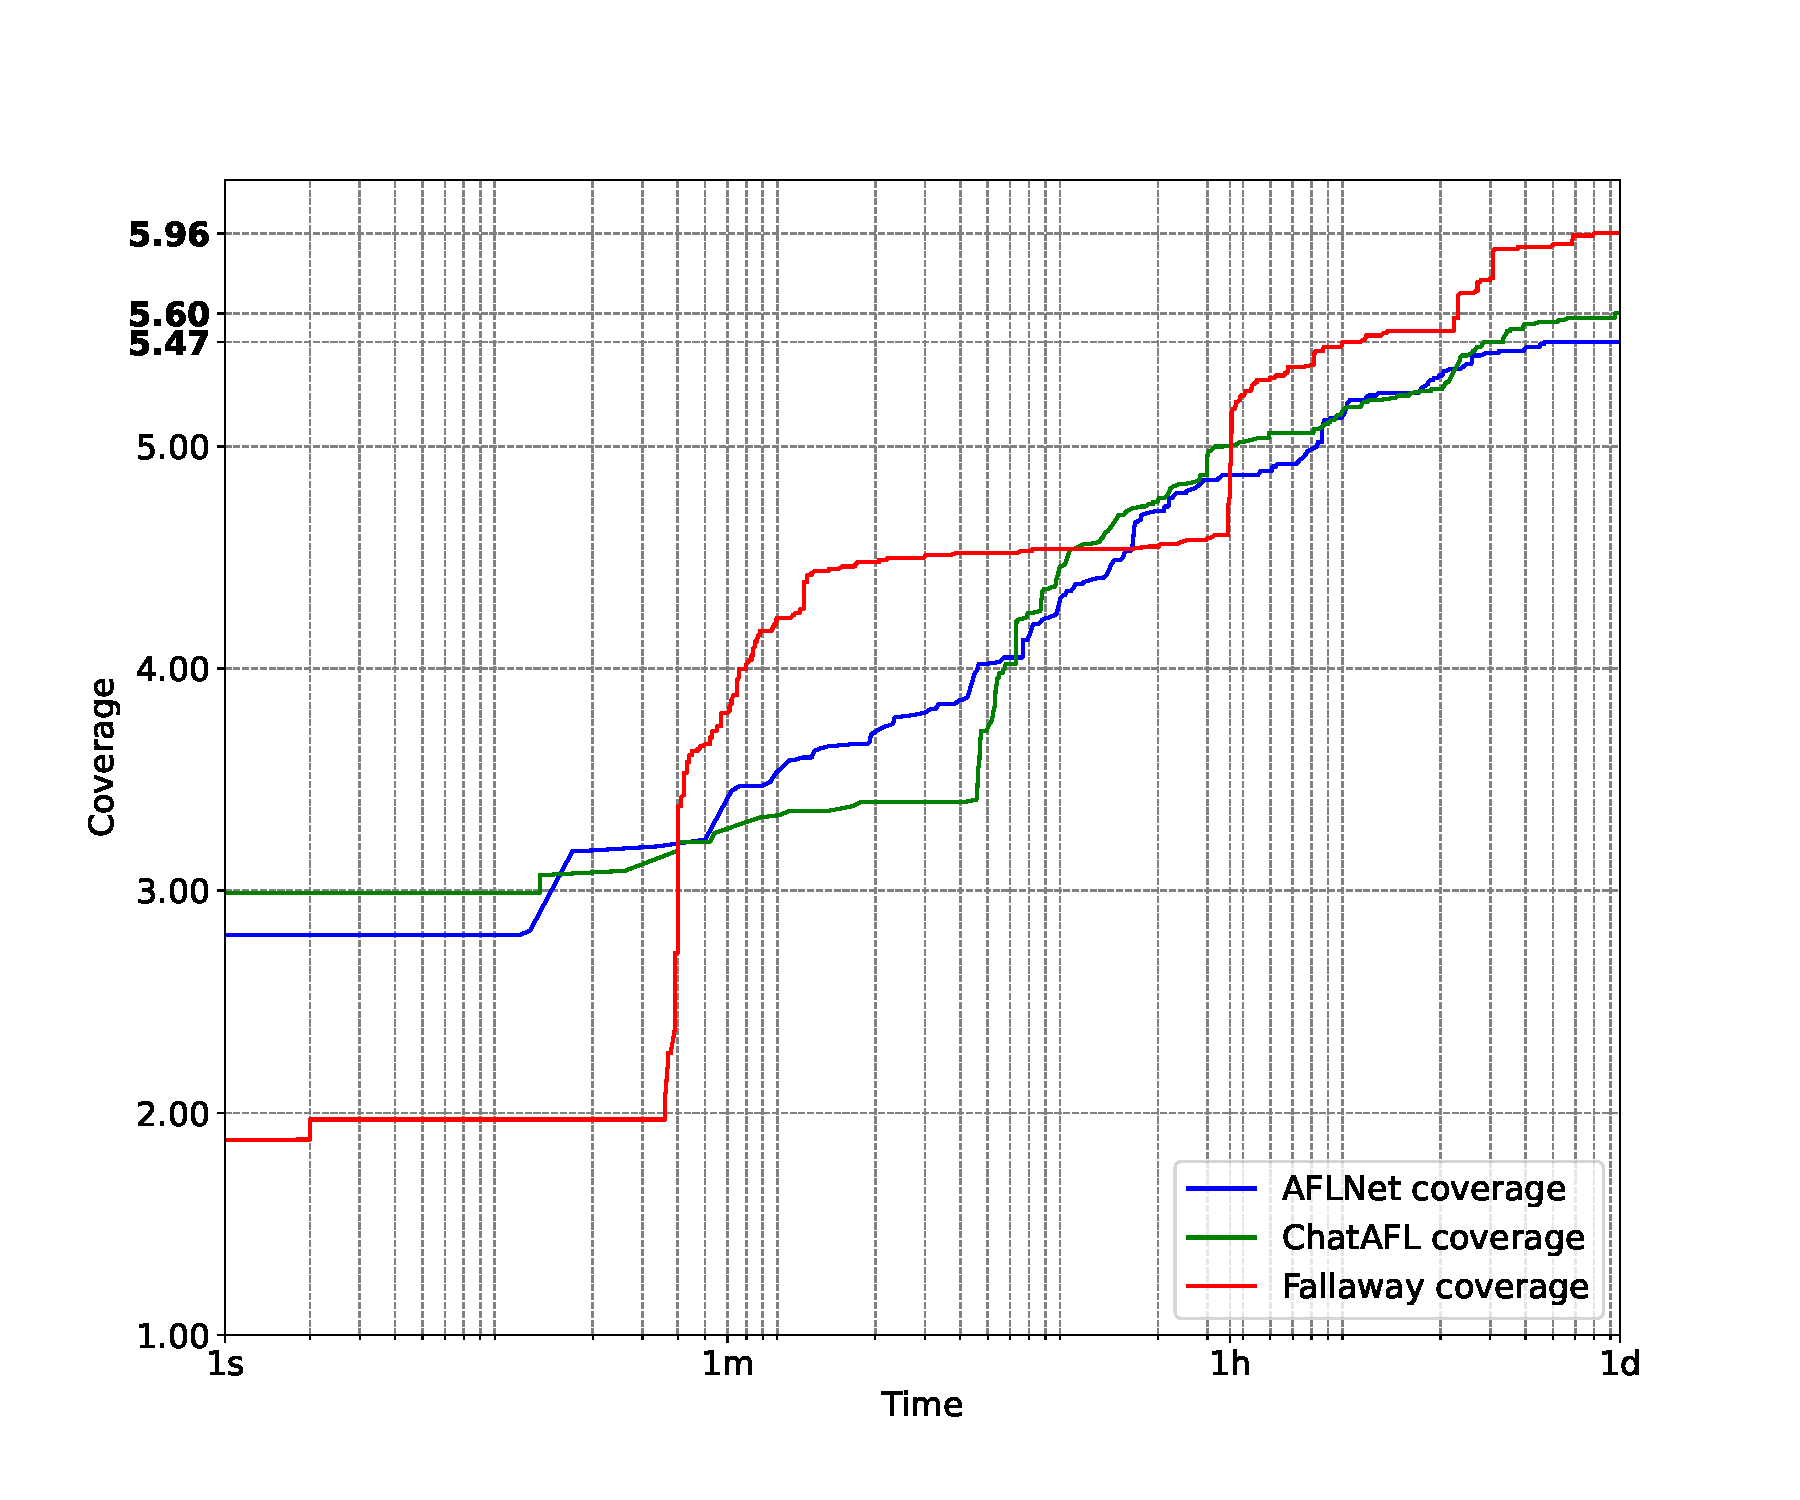
\includegraphics[width=1\textwidth]{Images/coverage_over_time_lighttpd-1day-2000l.pdf}
    \caption{Coverage of the three fuzzers in 24h with Fallaway in a loop of 2000}
    \label{fig:coverage_1day_2000l}
\end{figure}

\begin{figure}[H]
    \centering
    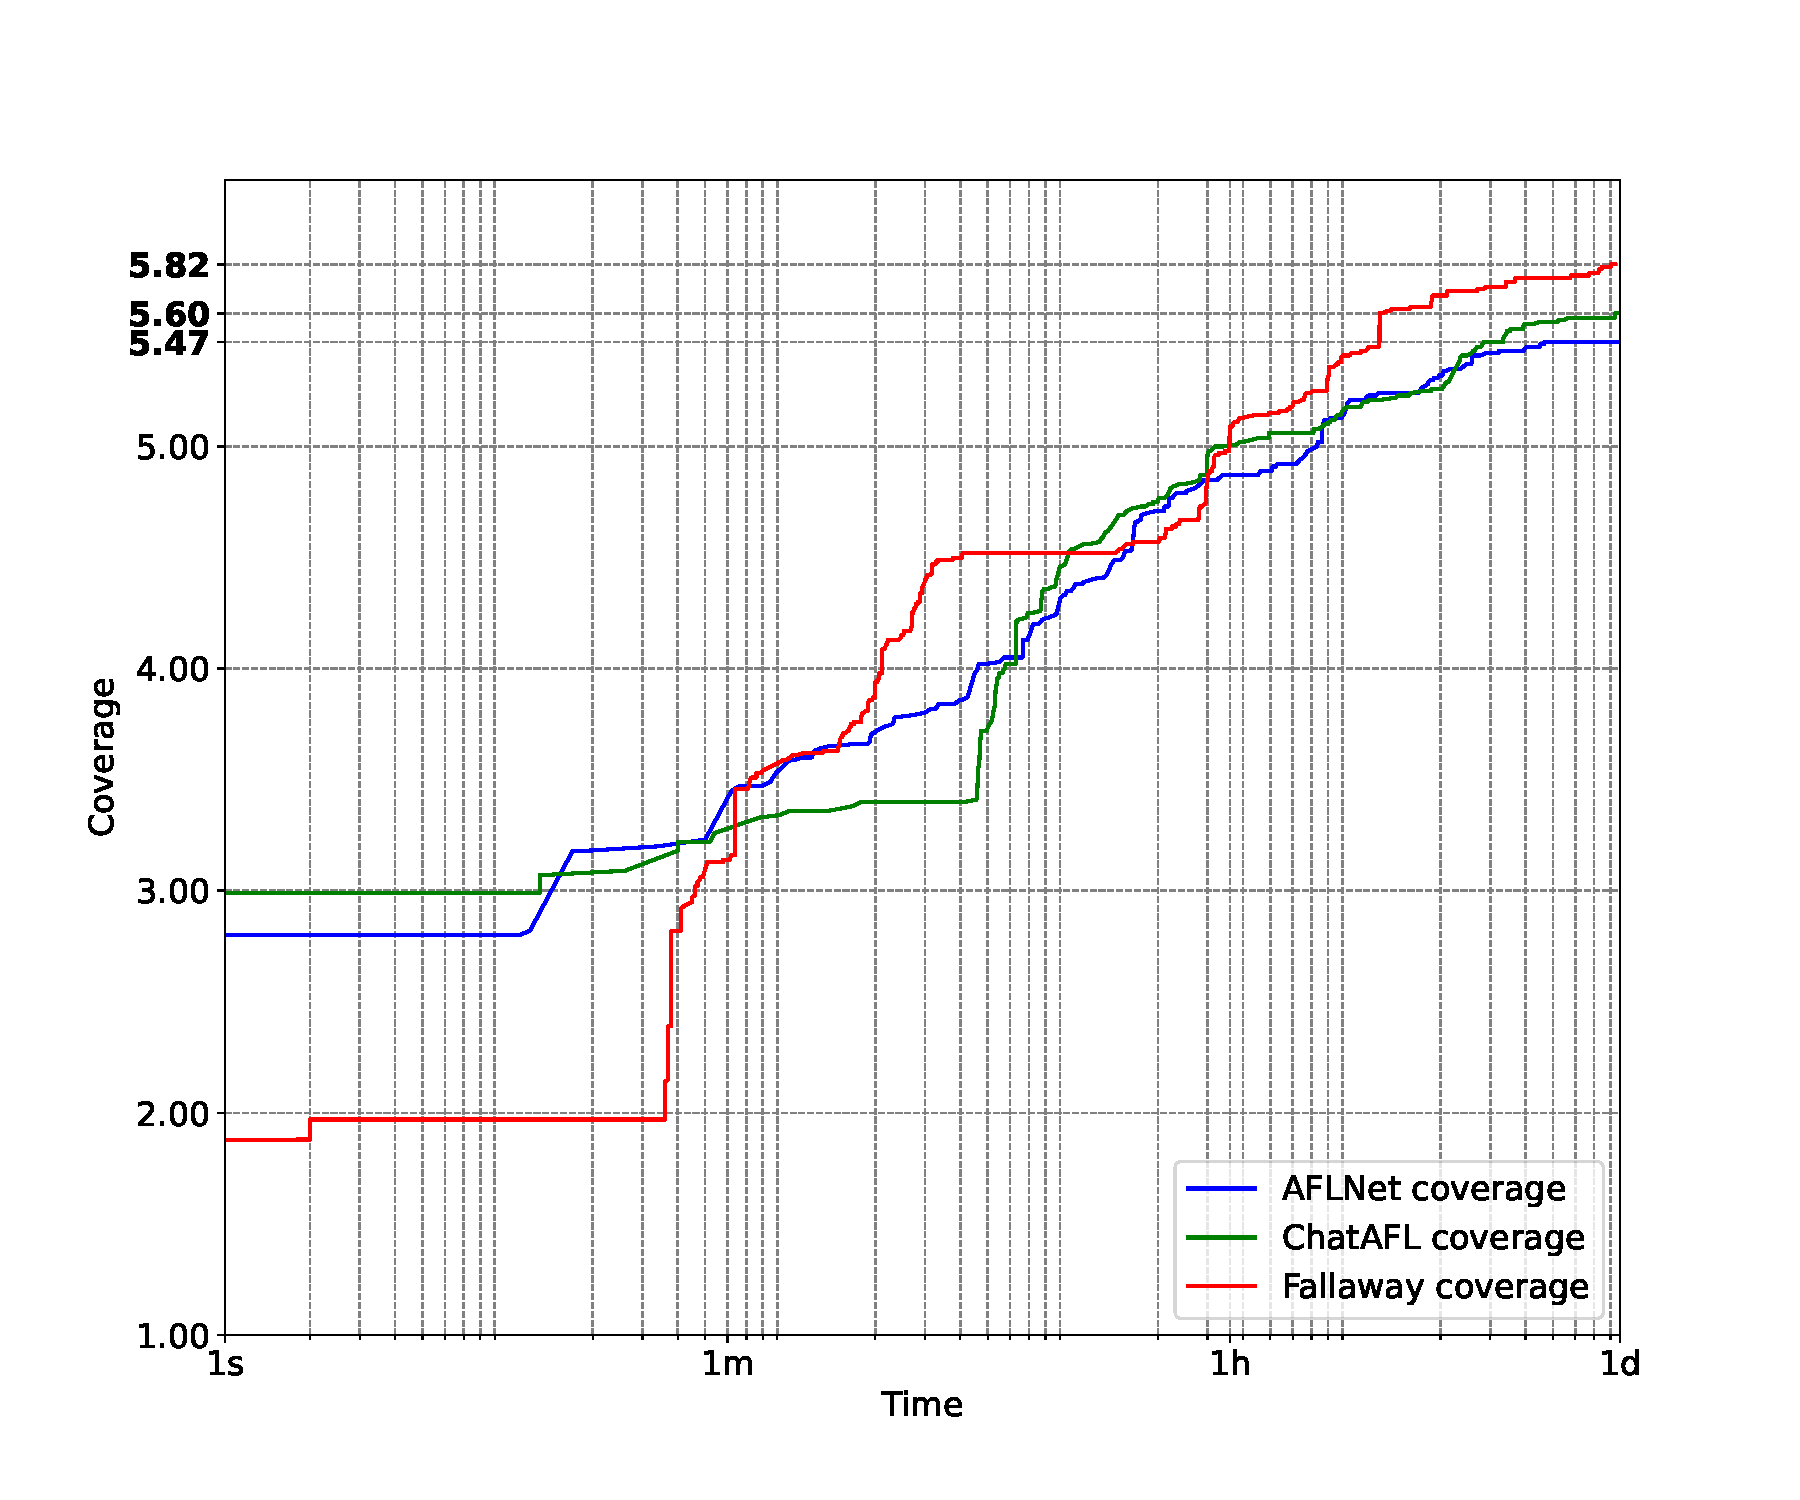
\includegraphics[width=1\textwidth]{Images/coverage_over_time_lighttpd-1day-1000l.pdf}
    \caption{Coverage of the three fuzzers in 24h with Fallaway in a loop of 1000}
    \label{fig:coverage_1day_1000l}
\end{figure}

\begin{figure}[H]
    \centering
    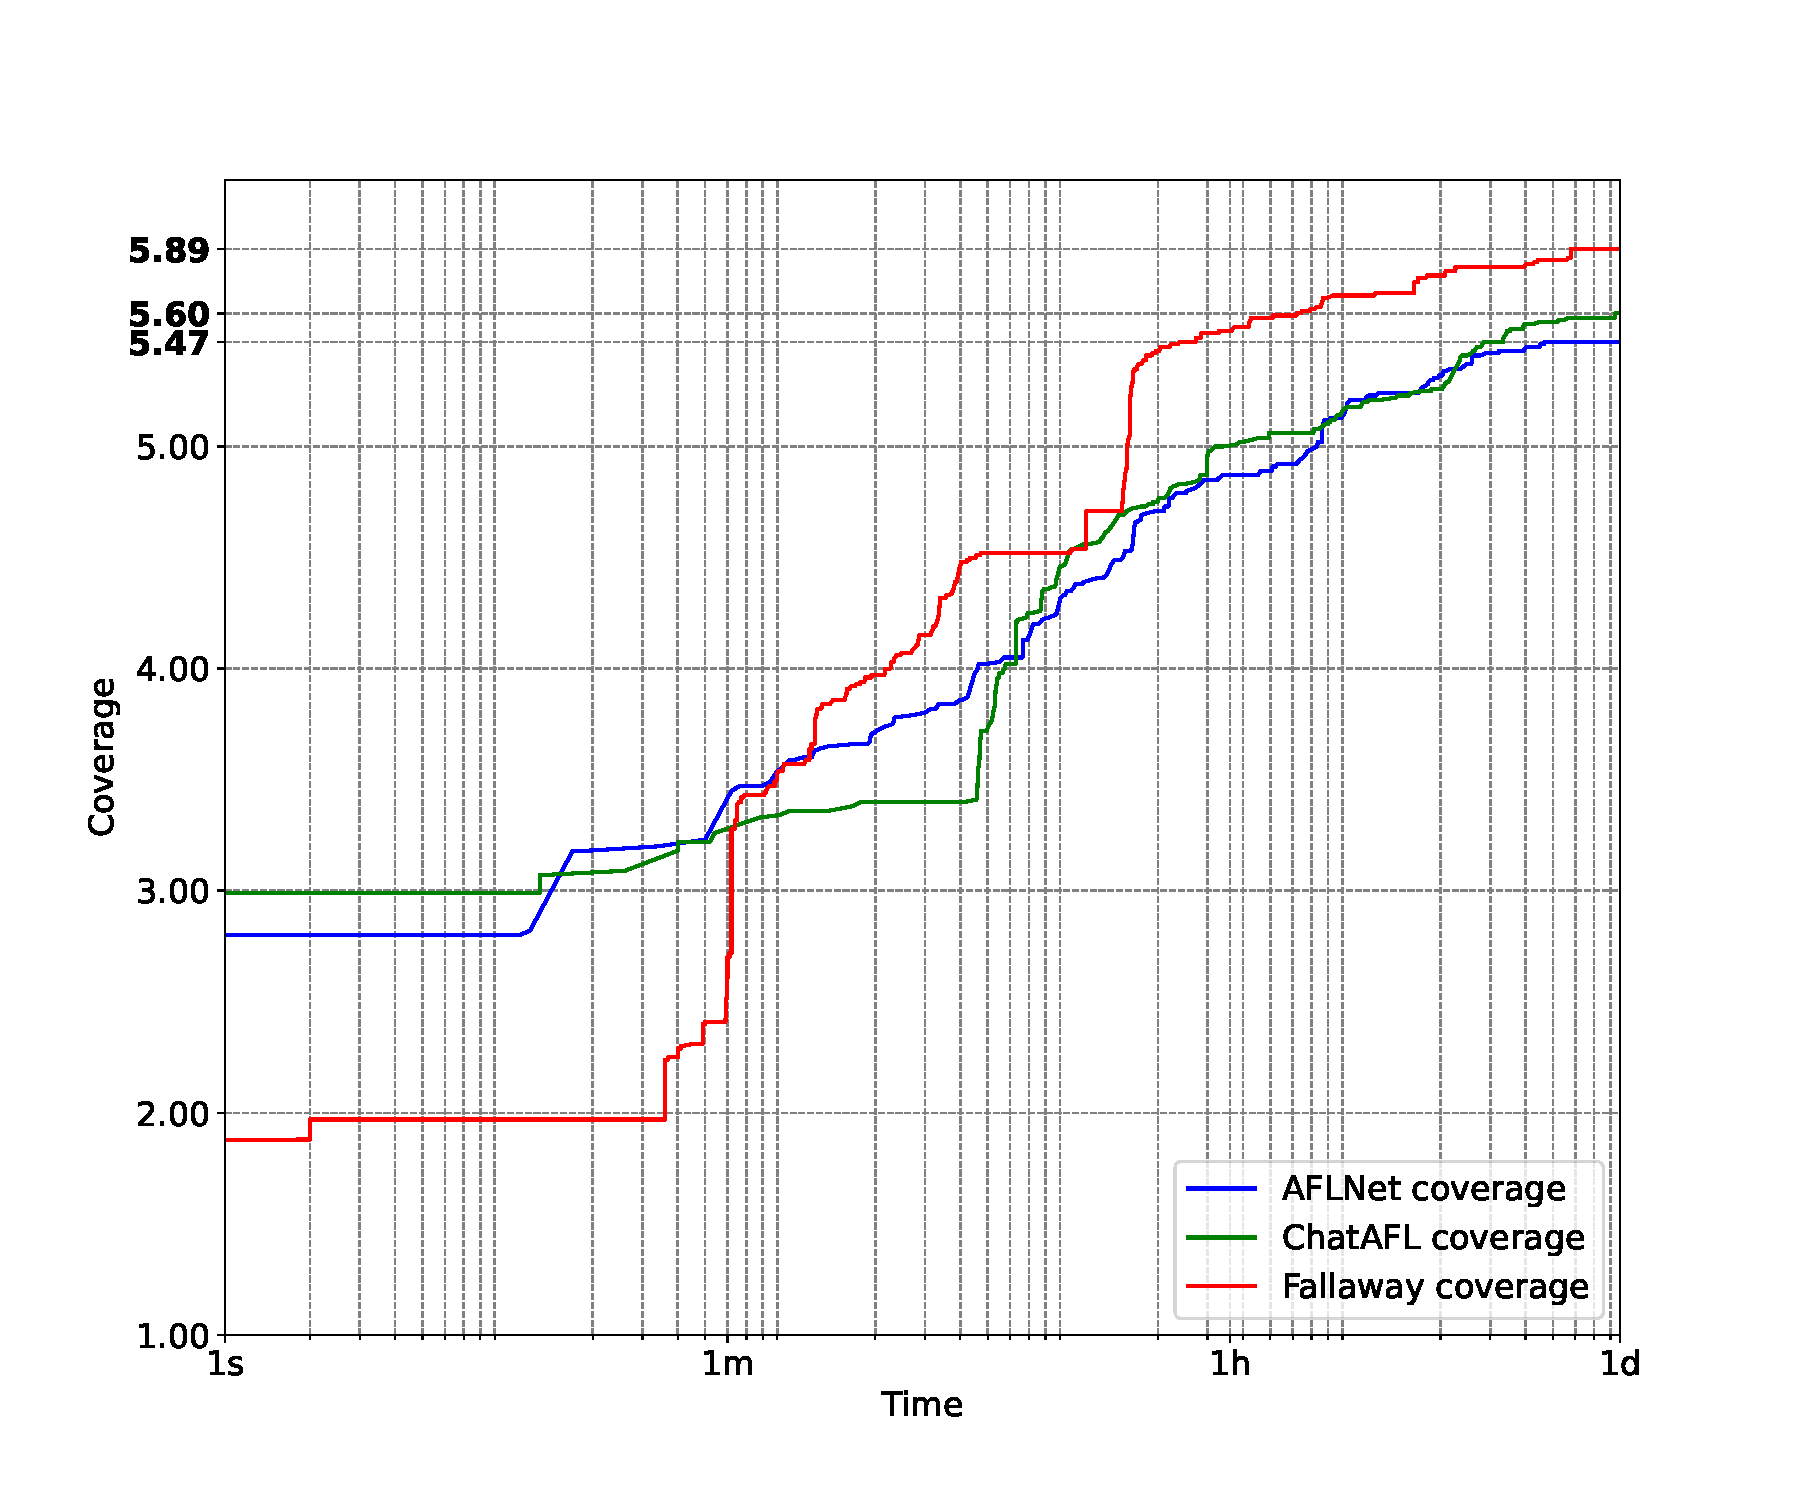
\includegraphics[width=1\textwidth]{Images/coverage_over_time_lighttpd-1day-500l.pdf}
    \caption{Coverage of the three fuzzers in 24h with Fallaway in a loop of 500}
    \label{fig:coverage_1day_500l}
\end{figure}

\begin{figure}[H]
    \centering
    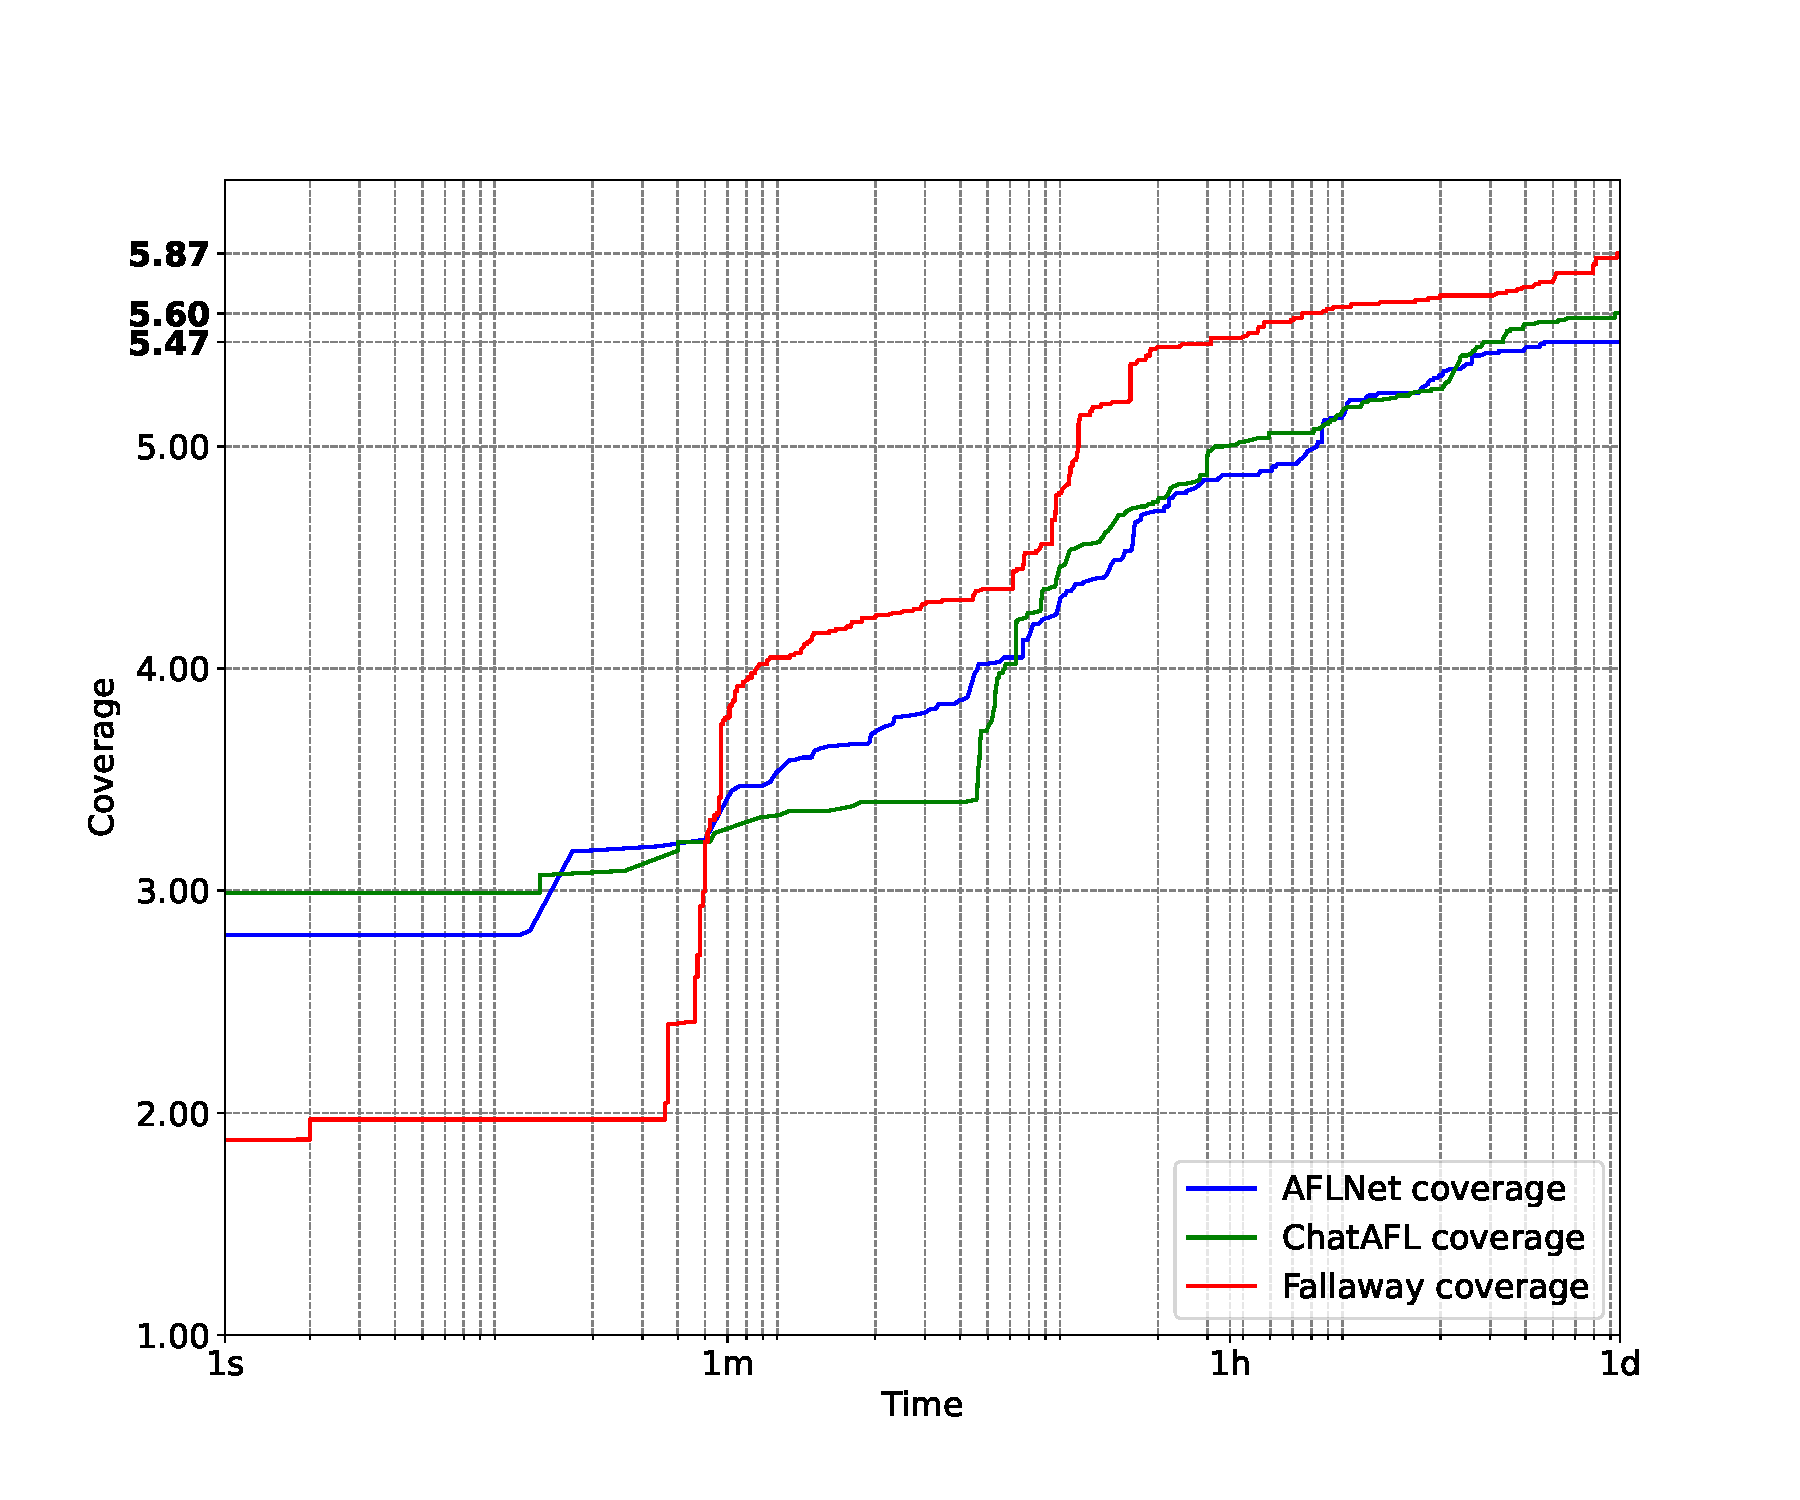
\includegraphics[width=1\textwidth]{Images/coverage_over_time_lighttpd-1day-250l.pdf}
    \caption{Coverage of the three fuzzers in 24h with Fallaway in a loop of 250}
    \label{fig:coverage_1day_250l}
\end{figure}

\begin{figure}[H]
    \centering
    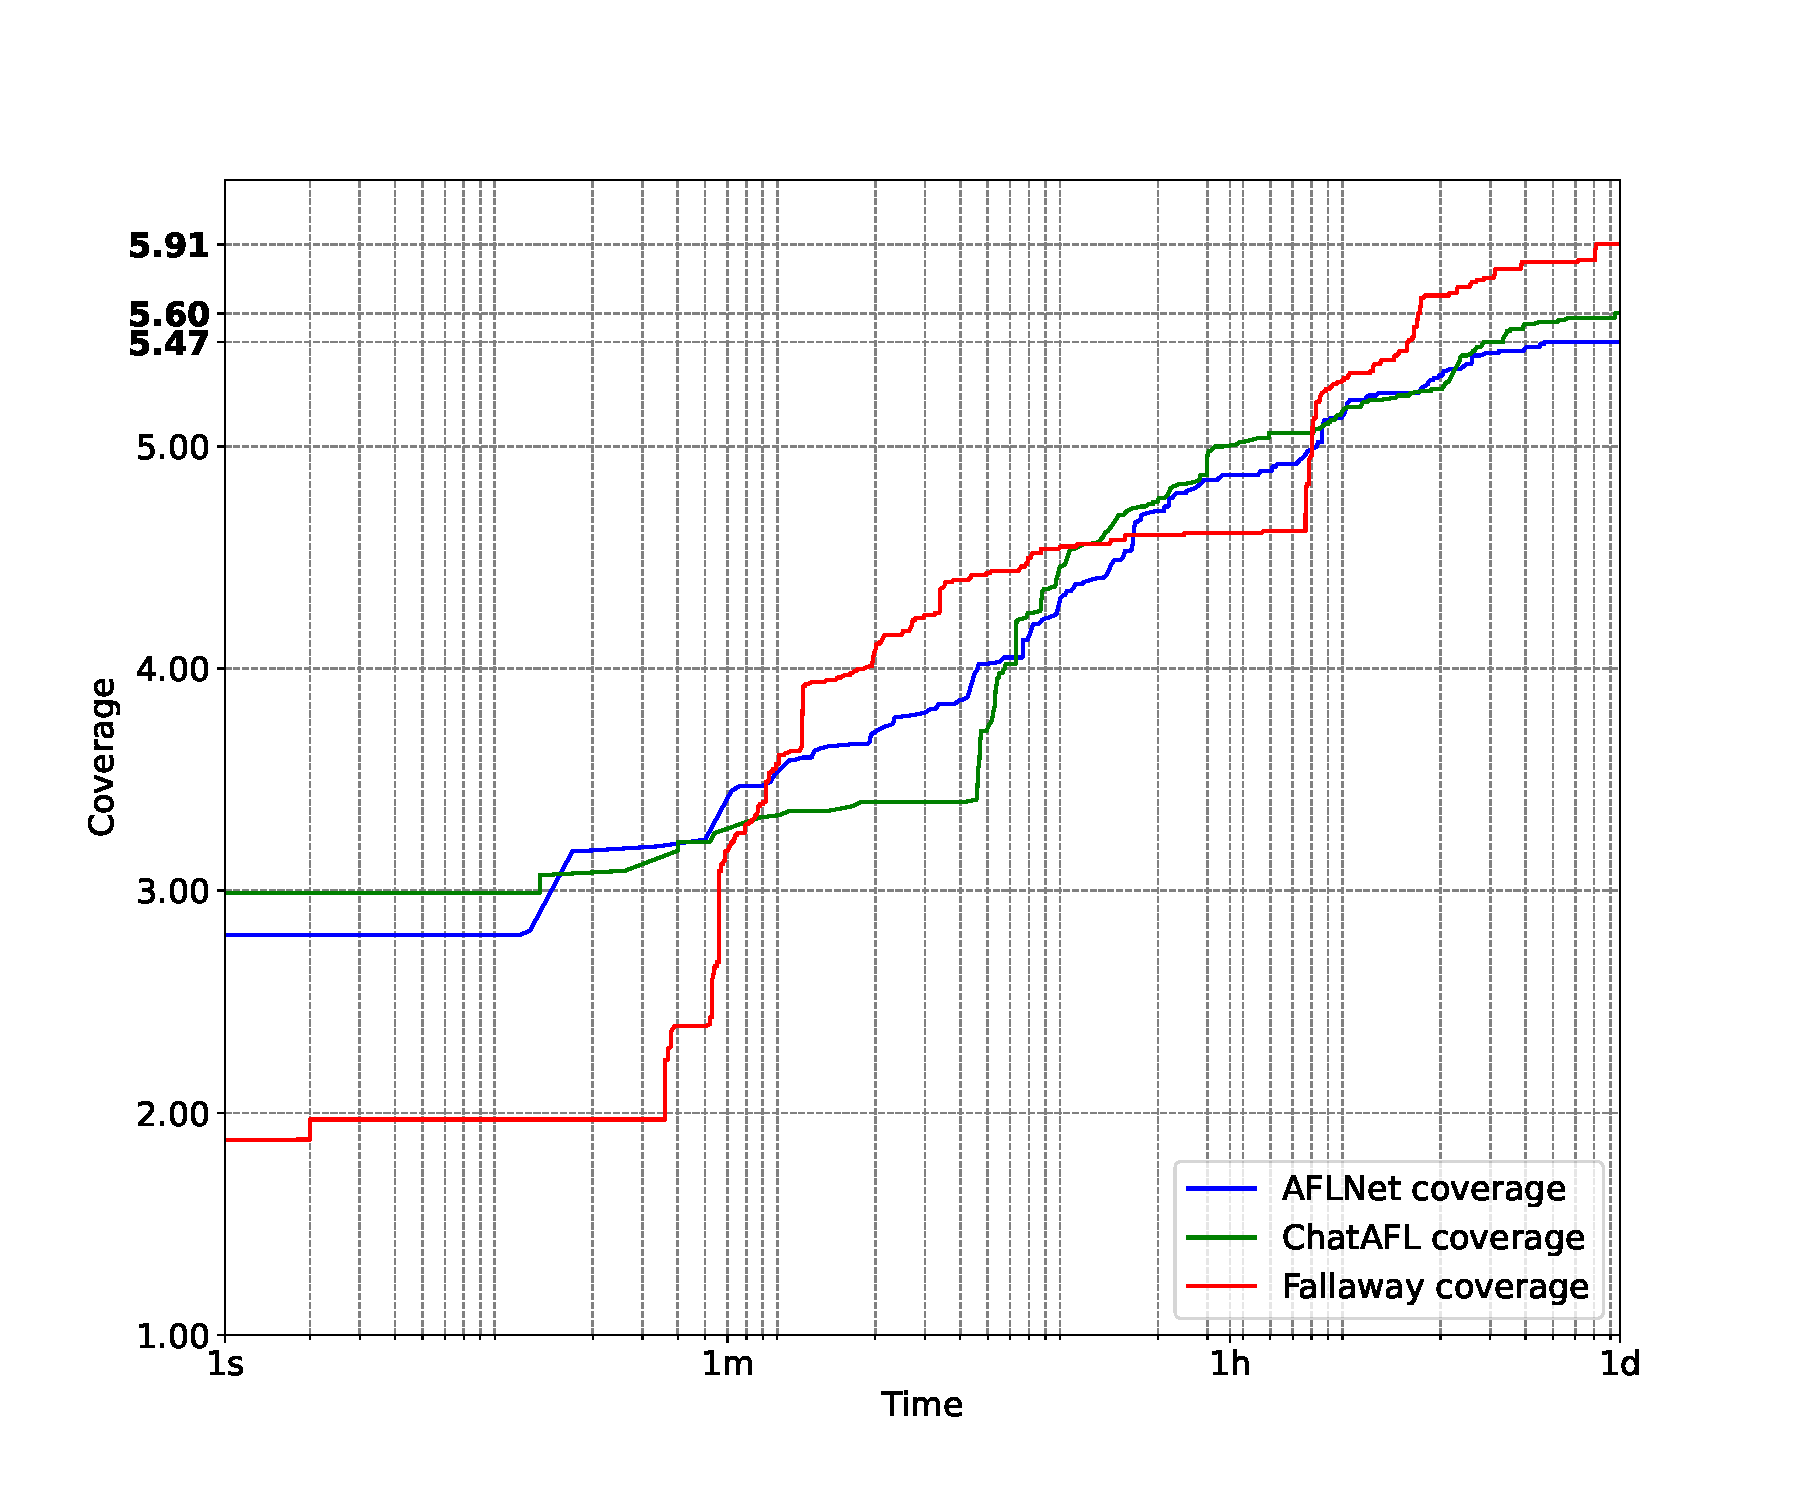
\includegraphics[width=1\textwidth]{Images/coverage_over_time_lighttpd-1day-100l.pdf}
    \caption{Coverage of the three fuzzers in 24h with Fallaway in a loop of 100}
    \label{fig:coverage_1day_100l}
\end{figure}

\begin{figure}[H]
    \centering
    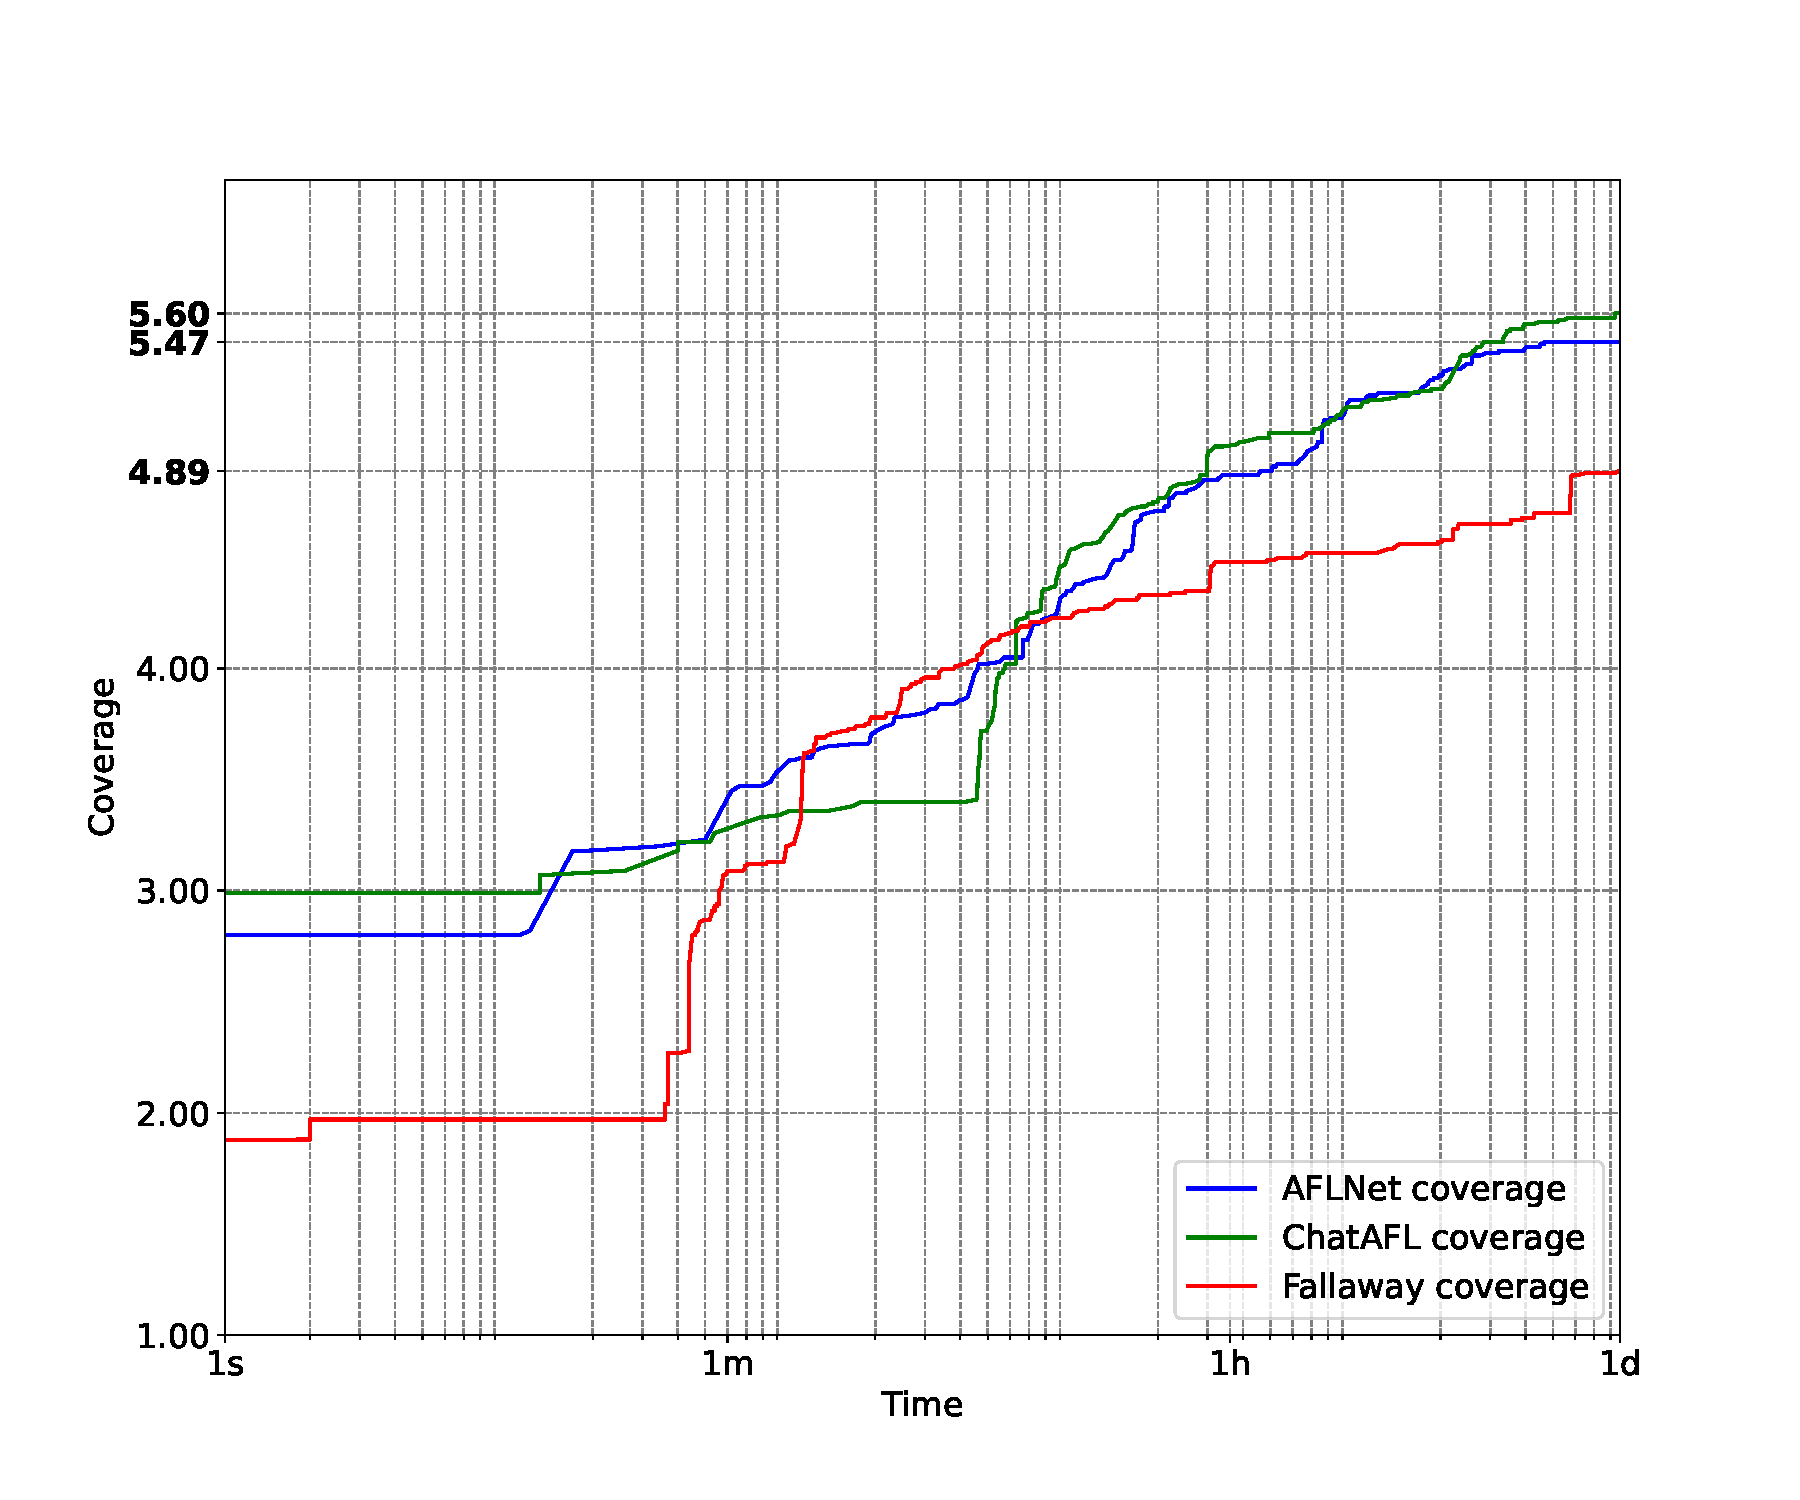
\includegraphics[width=1\textwidth]{Images/coverage_over_time_lighttpd-1day-10l.pdf}
    \caption{Coverage of the three fuzzers in 24h with Fallaway in a loop of 10}
    \label{fig:coverage_1day_10l}
\end{figure}
\phantom{}\\
As shown in Figure \ref{fig:coverage_1day_2000l}, Fallaway with a loop count of 2000 achieves the highest coverage. This is likely because the fuzzer can execute more test cases before transitioning between states. The other configurations of Fallaway, excluding the one with 10 loops, exhibit a similarly lower coverage, averaging around 5.87\%.
\\Although the loop counts differ, the coverage does not change significantly. This may be due to the implemented state model, which only considers two states: the existence or non-existence of a resource. As a result, even if the number of loops — and thus the number of possible test cases before changing states — varies, the coverage remains relatively stable. This limitation could be addressed by defining a more refined state model that includes additional states.
\\Figure \ref{fig:coverage_1day_10l} shows the lowest coverage at 4.89\%. In this scenario, the low loop count suggests a minimal number of possible test cases before switching states, which reduces the likelihood of extensive exploration.
\\In general, higher loop values can lead to increased coverage but may also result in redundant test cases and getting stuck in states with limited progress. Conversely, lower loop values can reduce coverage but also minimize redundancy and allow for faster progress.
\\Additionally, Fallaway does not exhibit linear growth in coverage; instead, it shows a more random behavior, even though its approach yields the best results observed. In contrast, AFLNet and ChatAFL demonstrate more linear growth in coverage, which indicates greater efficiency in code exploration. They start with higher initial coverage than Fallaway, suggesting they are better at targeting diverse code paths.
\\AFLNet achieves a coverage of 5.47\% with significantly fewer executions compared to Fallaway’s configurations, even those with a higher loop count (100 loops). ChatAFL reaches 5.60\% coverage with a number of executions similar to AFLNet. As ChatAFL is based on AFLNet, it effectively surpasses the coverage plateau observed with AFLNet.
\\An important thing to compare is the fact that AFLNet and ChatAFL consider executions as full traces
